\section{Requirements}
\label{sec:Requirements}
%openCV, bmob
\subsection{Overview} 
\paragraph{}
The Gift Box Project was conceived by Dr. Hunt from the the very popular game Pokemon Go. For this project, Dr. Hunt served as the supervisor.
\par The project initially included the development of the image comparator. However, the scope of the image comparator was too large and imposed too much complexity on the developer. To address this complexity, the developer, with assistance from Dr. Hunt, decided to use third-party software packages which would be able to perform the functionalities of image recognition. A software package was chosen depending on the required features. The scope of the program was therefore appropriately reduced by using the third-party software for the complex image recognition. The supervisor met with the developer several times to gather informal functional requirements of this program. These informal functional requirements helped to define the scope of the program as well as capture the true nature and purpose of the application. During the first of these informal meetings, the supervisor provided samples of the processed pictures with a wall-hanging and identified how to select a region. Based on the information collected from the meetings, the requirement document version 1.0 was created, in which the following fundamental requirements are listed:
\begin{itemize}
\item This project will support users with both web interface and Android application.
\item The virtual object sent by user can be selected from application or created by users. 
\item The attached object will fit the shape of region chosen by user.
\item The navigation can only support 2D locations. 
\item The image recognition will support image transformation including rotation, re-sizing and perspective removal
\item The algorithm will show a better result on images with strong features
\end{itemize}
\par Overall, the project produced two requirement documents. The requirement document version 1.0, included the detailed functional requirements described in Section 2.2. In version 2.0 of the requirement document we added a selected life cycle model, shown in
Section 2.3, as well as GUI requirements shown in Section 2.4.


\subsection{Functional Requirements}
\paragraph{}
This program leaves an administrator user type but it only supports one role, the System User for Android Application. Figure \ref{Use Cases Diagram} gives a Use Case diagram for the System User.
\par As shown in the Figure \ref{Use Cases Diagram}, there are eight use cases in the diagram. Each use case describes a functional requirement. These functional requirements are narrated as follows:

\begin{figure}[htb]
\centering
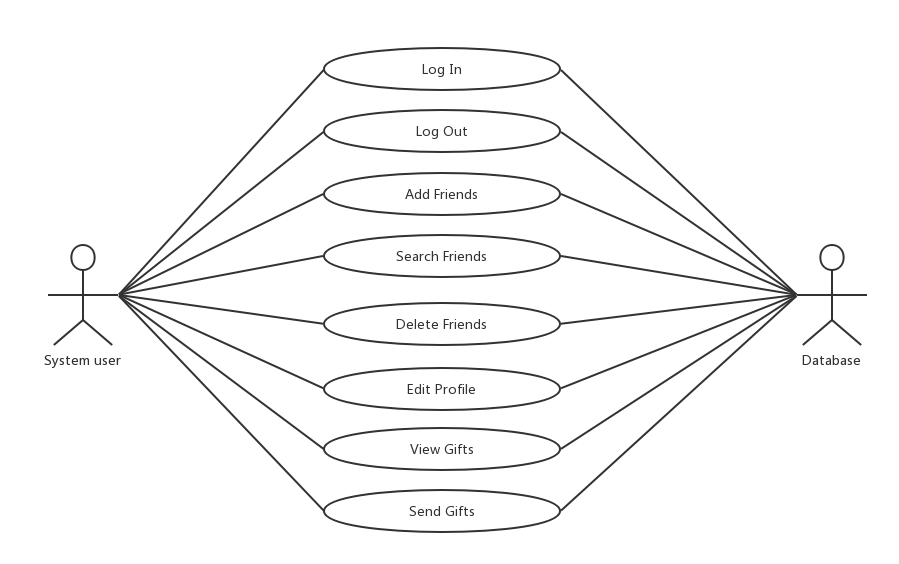
\includegraphics[width=.5\textwidth]{section02/assets/UseCase.png}
\caption[Short Caption 2]{\label{Use Cases Diagram}Use Case Diagram for Android}
\end{figure}

\begin{itemize}
\item The 'Log In' function allows users to log in to the system.
\item The 'Log Out' function allows users to log out of the system.
\item The 'Add Friends' function allows users to add other users as friends. This add function doesn't need other users' agreement.
\item The 'Search Friends' function allows users to search other users by username.
\item The 'Delete Friends' function allows users to delete friends from their friends list.
\item The 'Edit Profile' function allows users to edit their password and portrait information. The username and email cannot be changed after registration. 
\item The 'View Gifts' function allows users to view their gifts. Gifts are filtered based on 'Sent' or 'Received'.
\item The 'Send Gifts' function allows users to send virtual gifts to other users.
\end{itemize}
\par The web interface contains the same functionalities with Android application except 'Send Gifts' and it won't be able to view the not found gifts either.



\subsection{Selection of Life Cycle Model}
\paragraph{} We analyzed the requirements in requirement document version 1.0 and identified the risks listed below:
\begin{itemize}
\item Lack of detailed specification for the GUI.
\item Lack of experience on image recognition.
\item Potential misunderstanding between supervisor and developer.
\end{itemize}
\par These risks described above are roughly estimated based on the situations described by the supervisor and developer. To alleviate these risks, we determined to use an adaptive software development model. The incremental model is a method of software development where the model is designed, implemented and tested incrementally until the product is finished. Also as shown in Figure \ref{IncrmentalModel}, there are infinite additions possible for the product.
\par Compared to other models, this one will check the consistency between requirements in each reaction, most important functionalities are considered as and when they arrive, developers ensure that the product is partially ready with selected requirements and customers feel the progress of the development process.
\par As a result, each partial functionality can be checked in each interaction and will be able to get feedback for developing additional requirements in the next increment. Also, if there are changes made during the development system development would be able to response to these changes rapidly.

\begin{figure}[htb]
\centering
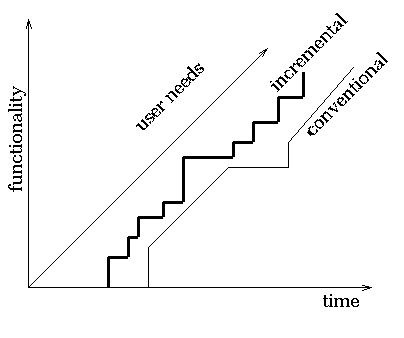
\includegraphics[width=.5\textwidth]{section02/assets/IncrementalModel.png}
\caption[Short Caption 2]{\label{IncrmentalModel}Graphical Illustration of Incremental Prototyping Model}
\end{figure}

\par Each increment includes the completion of several functional requirements. The major consideration to determining which functionalities should be included in the earlier seven increments is according to their importance and their contribution to the entire system development.
\par Functionalities concerning image recognition procedure  and image perspective should have a higher priority than others. The increments that occurred in this project are listed below:
\begin{itemize}
\item Increment 1: Graphical User Interface functionalities related to basic user interaction.
\item Increment 2: Image recognition's functionalities related to application interaction.
\item Increment 3: Image perspective functionalities related to application interaction.
\item Increment 4: Enhancing application review and evaluation.
\item Increment 5: System configuration.
\item Increment 6: Writing and executing test cases.
\item Increment 7: Enhancing interactivity of Graphical User Interface.
\end{itemize}

\subsection{GUI Functional Requirements}
The GUI functional requirements closely mirror the functional requirements. In version 2.0, the GUI shown in Figure 4, was designed based on the very first requirements of the project. However, the requirements of GUI were changed after some meetings with supervisor because of the modification of requirements.
\begin{figure}[H]
\centering
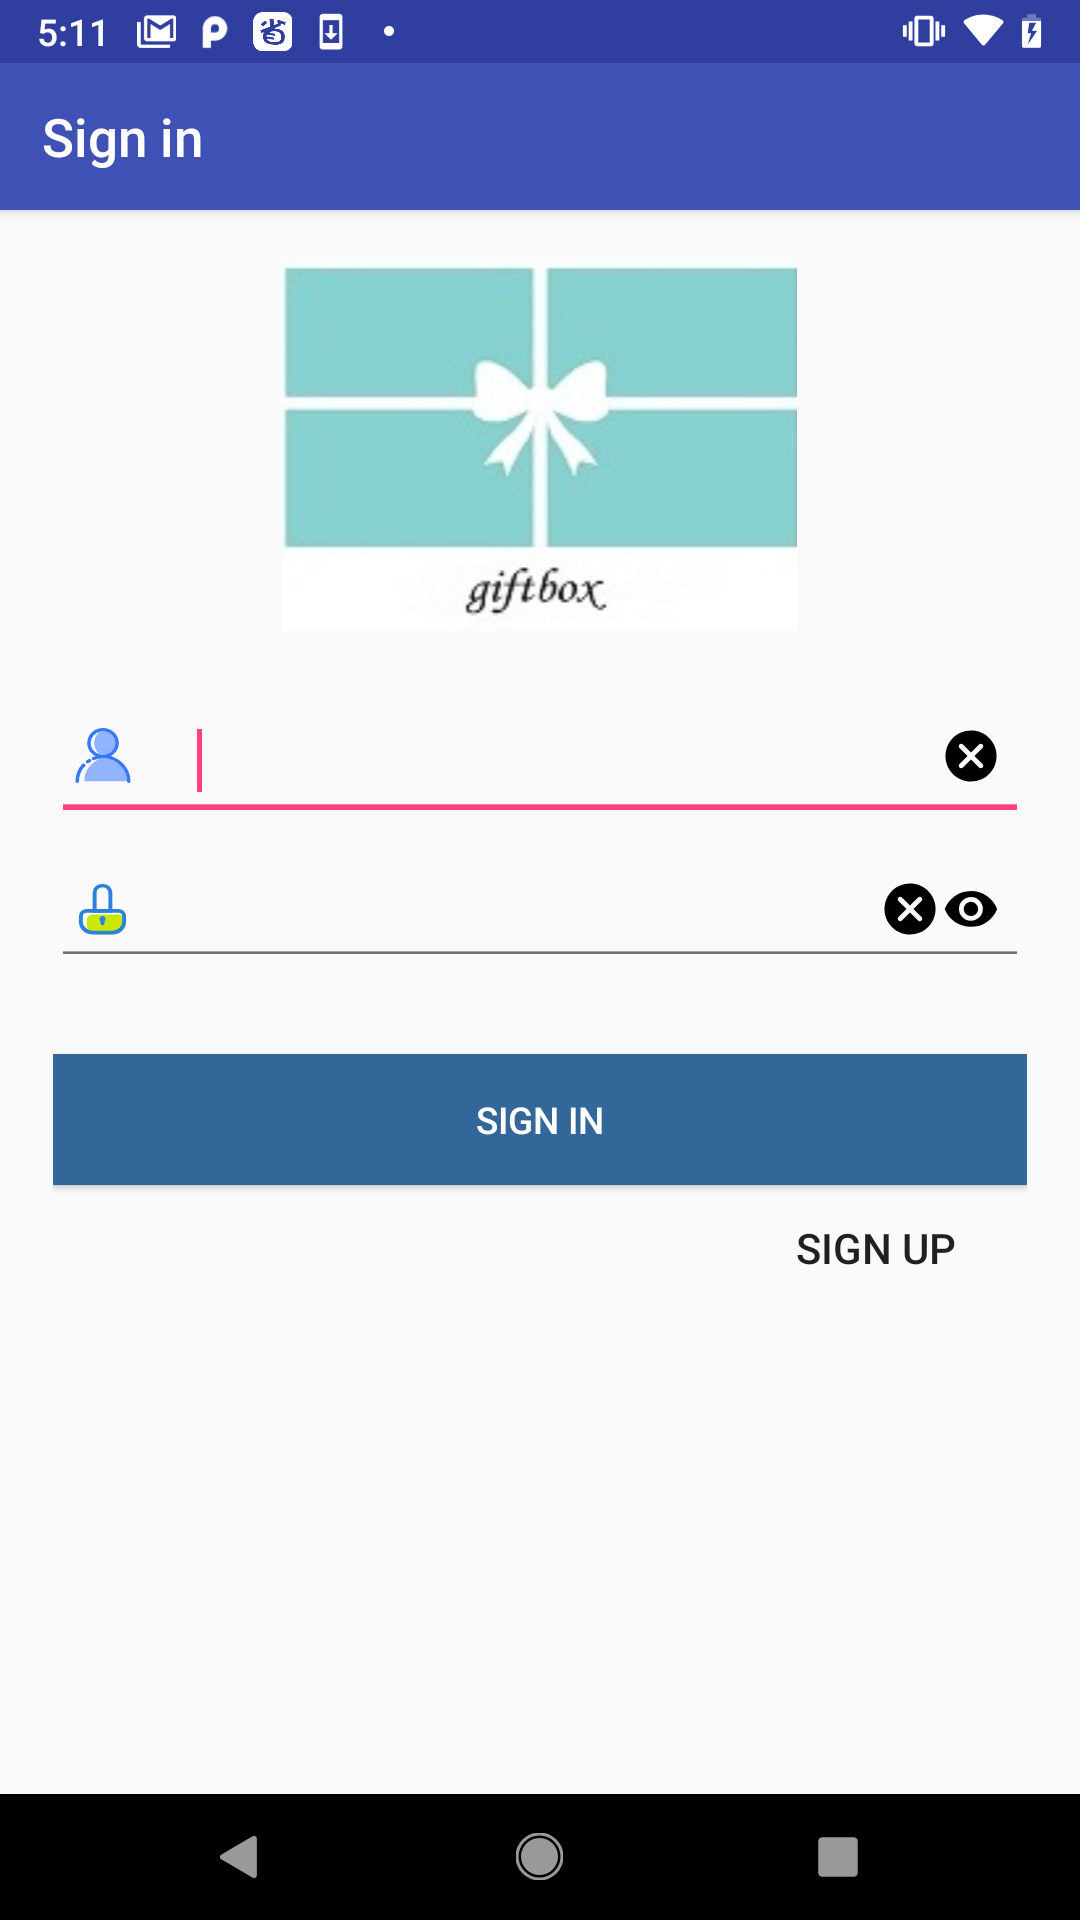
\includegraphics[width=.25\textwidth]{section02/assets/SignIn.png}
\caption[Short Caption 2]{\label{SignIn}Log In Page}
\end{figure}
\par Users can log in from this page, the 'eye' icon is able to switch the password between plain text and encrypted text.

\begin{figure}[H]
\centering
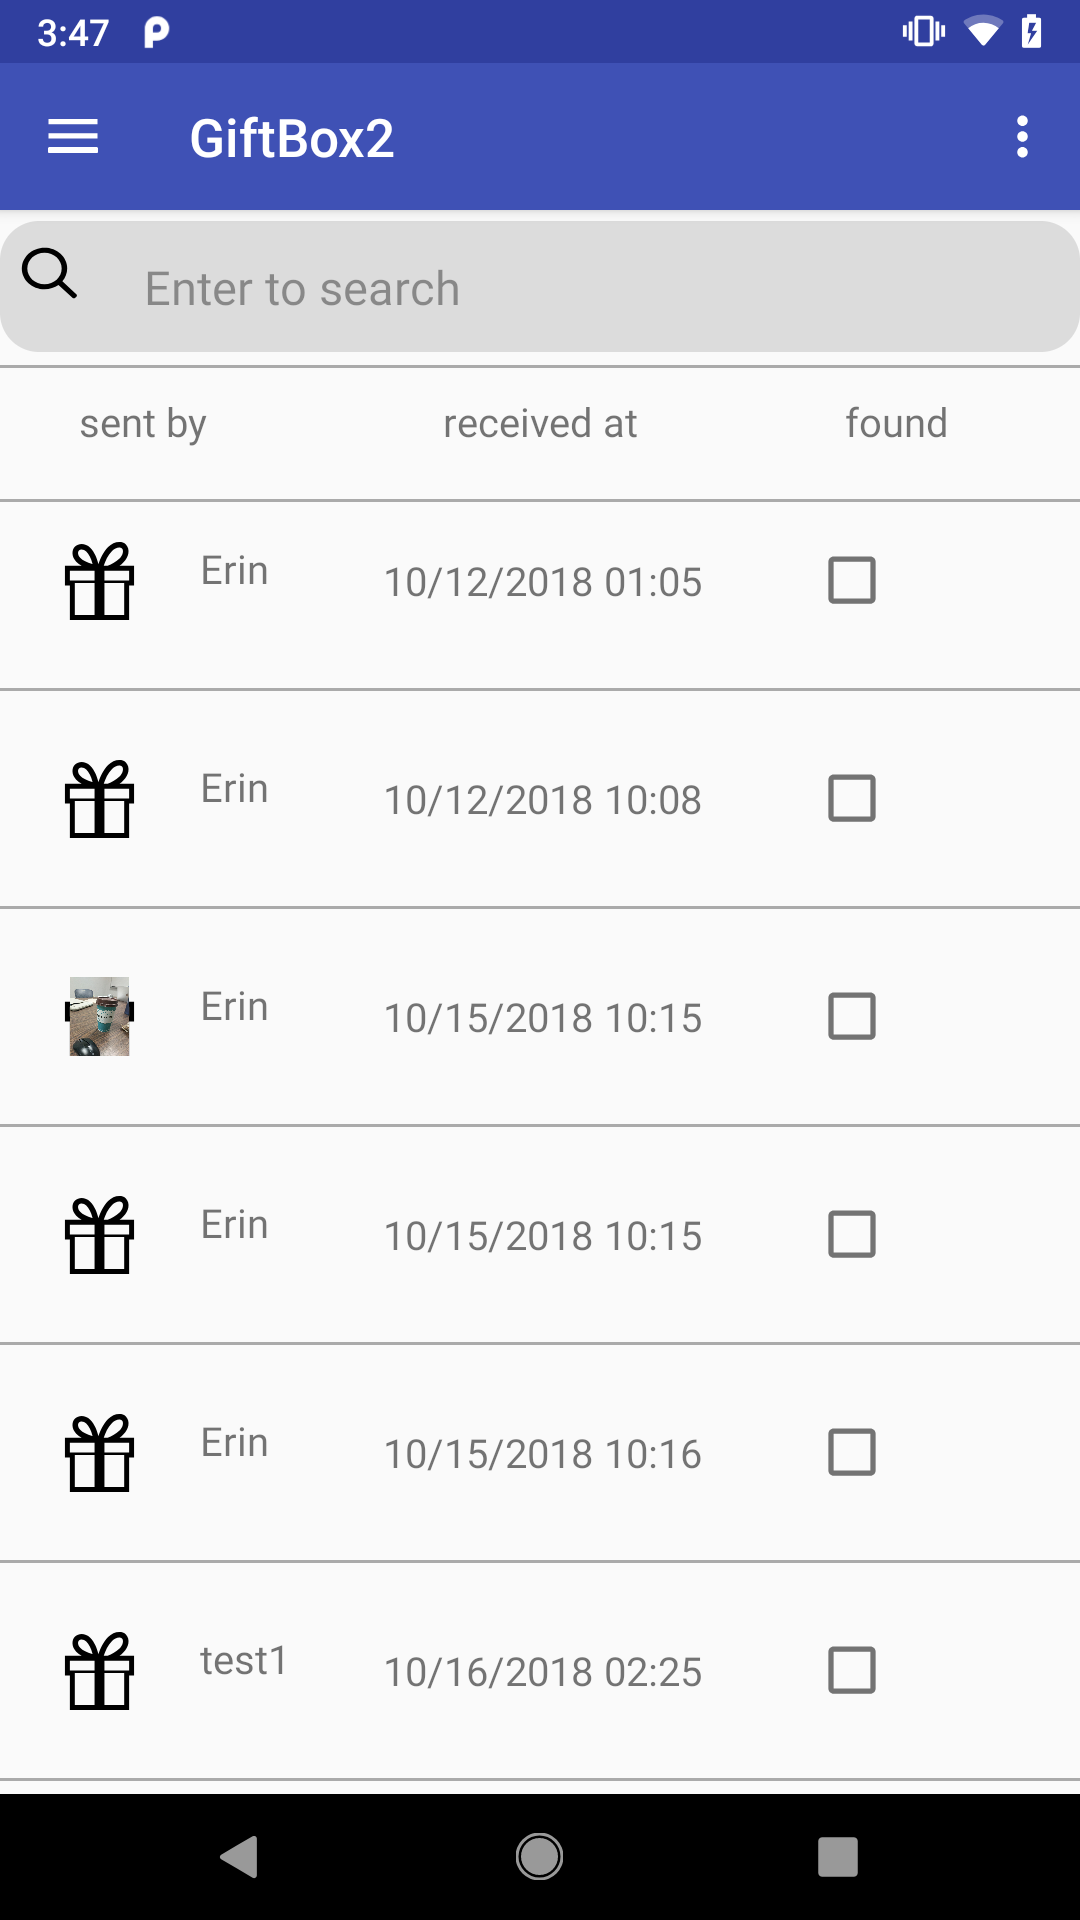
\includegraphics[width=.25\textwidth]{section02/assets/MainPage.png}
\caption[Short Caption 2]{\label{MainPage}Main Page}
\end{figure}
\par User will see the gifts they received after they log in. The top left corner button will help users to go to other functional pages. They can also change their portraits by clicking on the profile picture.

\begin{figure}[H]
\centering
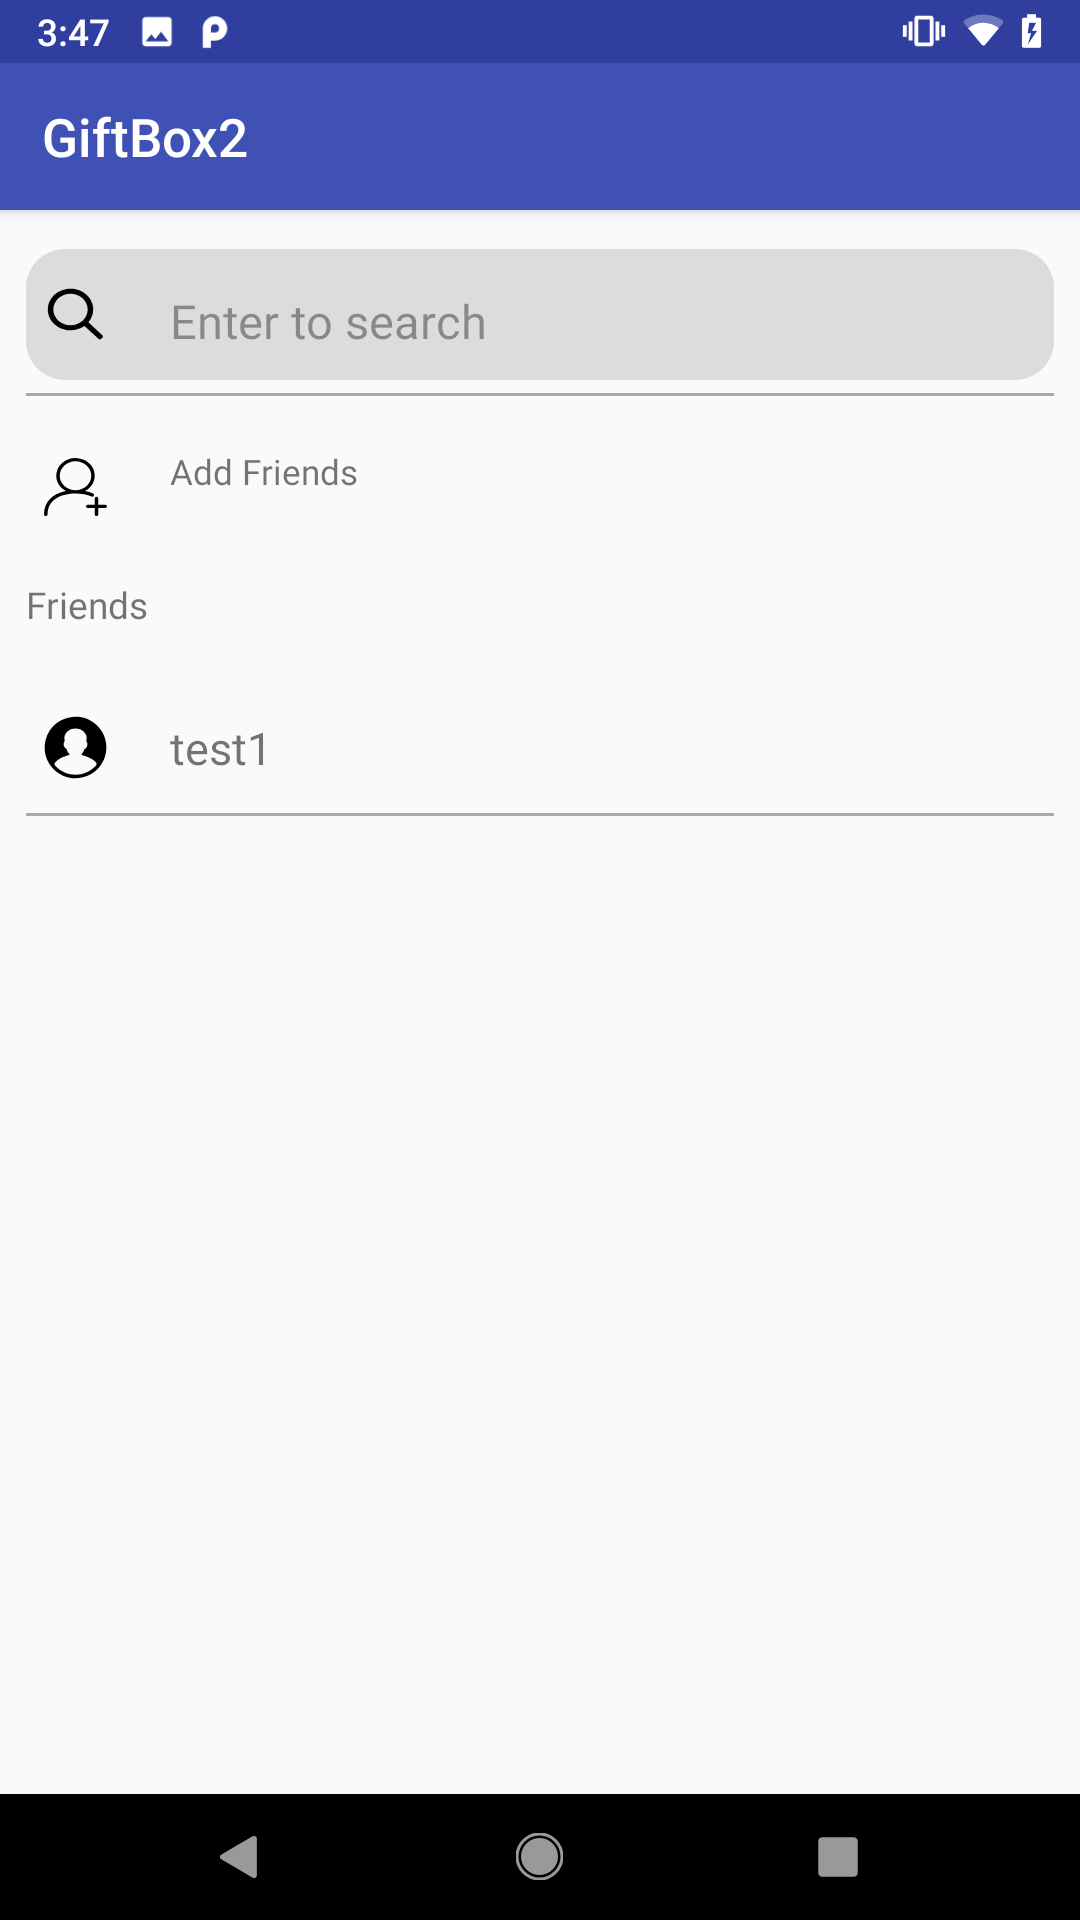
\includegraphics[width=.25\textwidth]{section02/assets/FriendsList.png}
\caption[Short Caption 2]{\label{FriendsList}Friends List Page}
\end{figure}
\par On the friends list page users can search their current friends at the search field. The 'Add Friends' button can let users add a new friend. Users can also delete friends and send gifts by a long click on different users.

\begin{figure}[H]
\centering
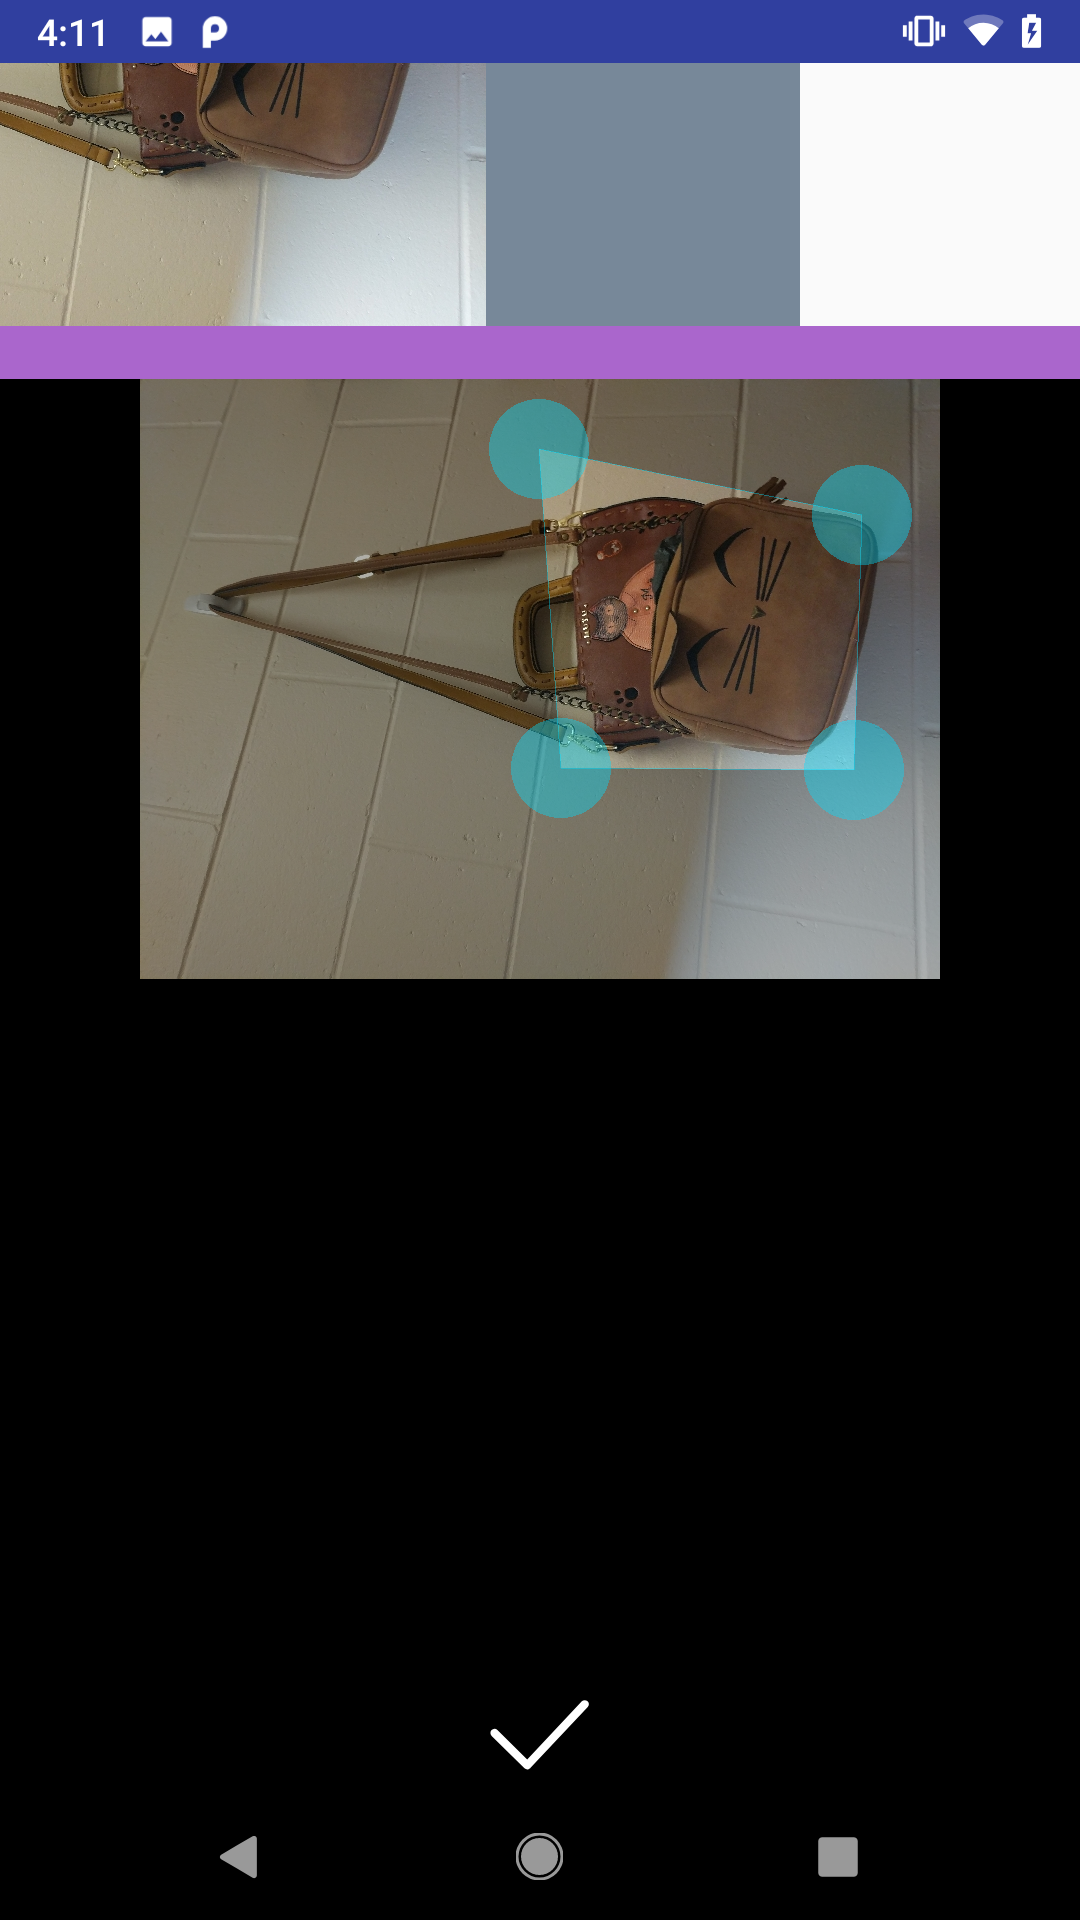
\includegraphics[width=.25\textwidth]{section02/assets/SendGift.png}
\caption[Short Caption 2]{\label{SendGift}Send Gift Page}
\end{figure}
\par Users can select any shape of region to attach a gift and send to the chosen recipient.

 
